\documentclass[10pt,xcolor=pdflatex]{beamer}
\usepackage{newcent}
\usepackage[utf8]{inputenc}
%\usepackage[czech]{babel}
\usepackage{hyperref}
\usepackage{fancyvrb}
\usepackage{multicol}
\usetheme{FIT}

%%%%%%%%%%%%%%%%%%%%%%%%%%%%%%%%%%%%%%%%%%%%%%%%%%%%%%%%%%%%%%%%%%
\title[]{Counting People Using a PIR Sensor}

\author[]{Martin Beneš}

\institute[]{Brno University of Technology, Faculty of Information Technology\\
Božetěchova 1/2. 612 66 Brno - Královo Pole\\
xbenes49@stud.fit.vutbr.cz}

%\date{January 1, 2016}
\date{\today}
%\date{} % bez data

%%%%%%%%%%%%%%%%%%%%%%%%%%%%%%%%%%%%%%%%%%%%%%%%%%%%%%%%%%%%%%%%%%

\begin{document}

\frame[plain]{\titlepage}


% ---- AIM ---- %
\begin{frame}\frametitle{The aim}
    \begin{itemize}
        \item Study the topic.
        \item Design a theoretical system, that could:
            \begin{itemize}
                \item \emph{Localize} a person.
                \item Estimate \emph{a count} of people.
            \end{itemize}
        \item Implement and test the approach.
        \item Summarize.
    \end{itemize}
\end{frame}

% ---- DESIGN ---- %
\begin{frame}\frametitle{The design}
    \begin{itemize}
        \item Sensor device (PIR STD, NodeMCU)
            \begin{itemize}
                \item Sampling
            \end{itemize}
        \item Classification server (Python, NumPy)
            \begin{itemize}
                \item Classification
                \item Fusion
            \end{itemize}
    \end{itemize}

    \begin{center}
        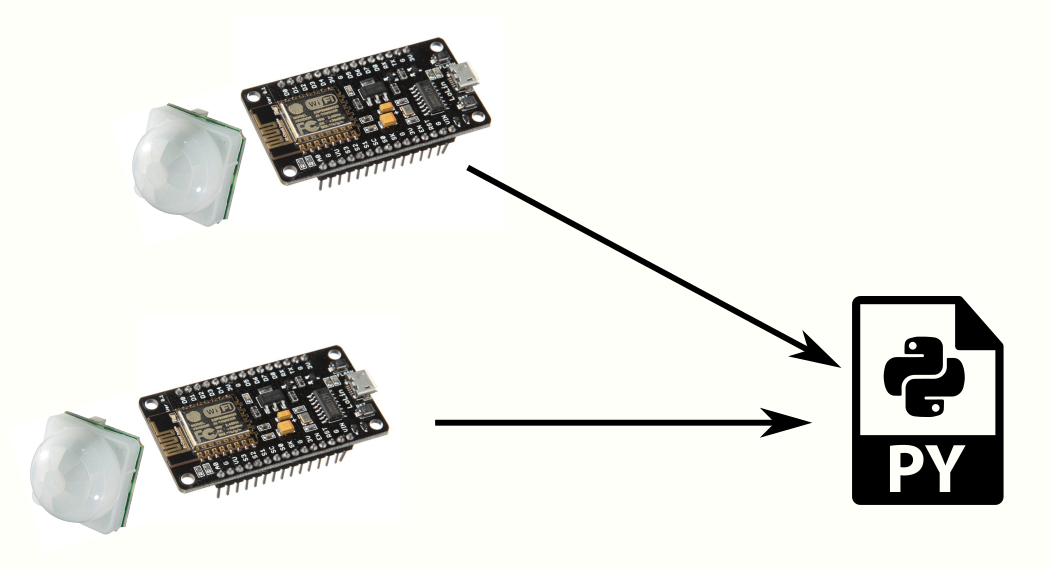
\includegraphics[width=0.7\textwidth]{img/structure.png}
    \end{center}
\end{frame}

% ---- FEATURE EXTRACTION ---- %
\begin{frame}\frametitle{Classification: feature extraction}
    \begin{center}
        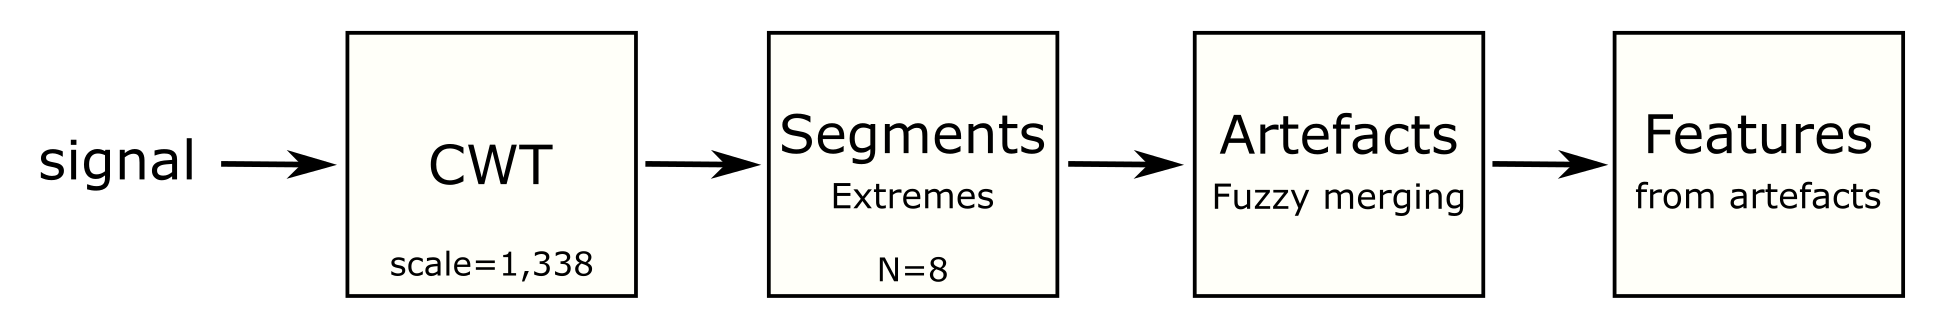
\includegraphics[width=1\textwidth]{img/features2.png}

        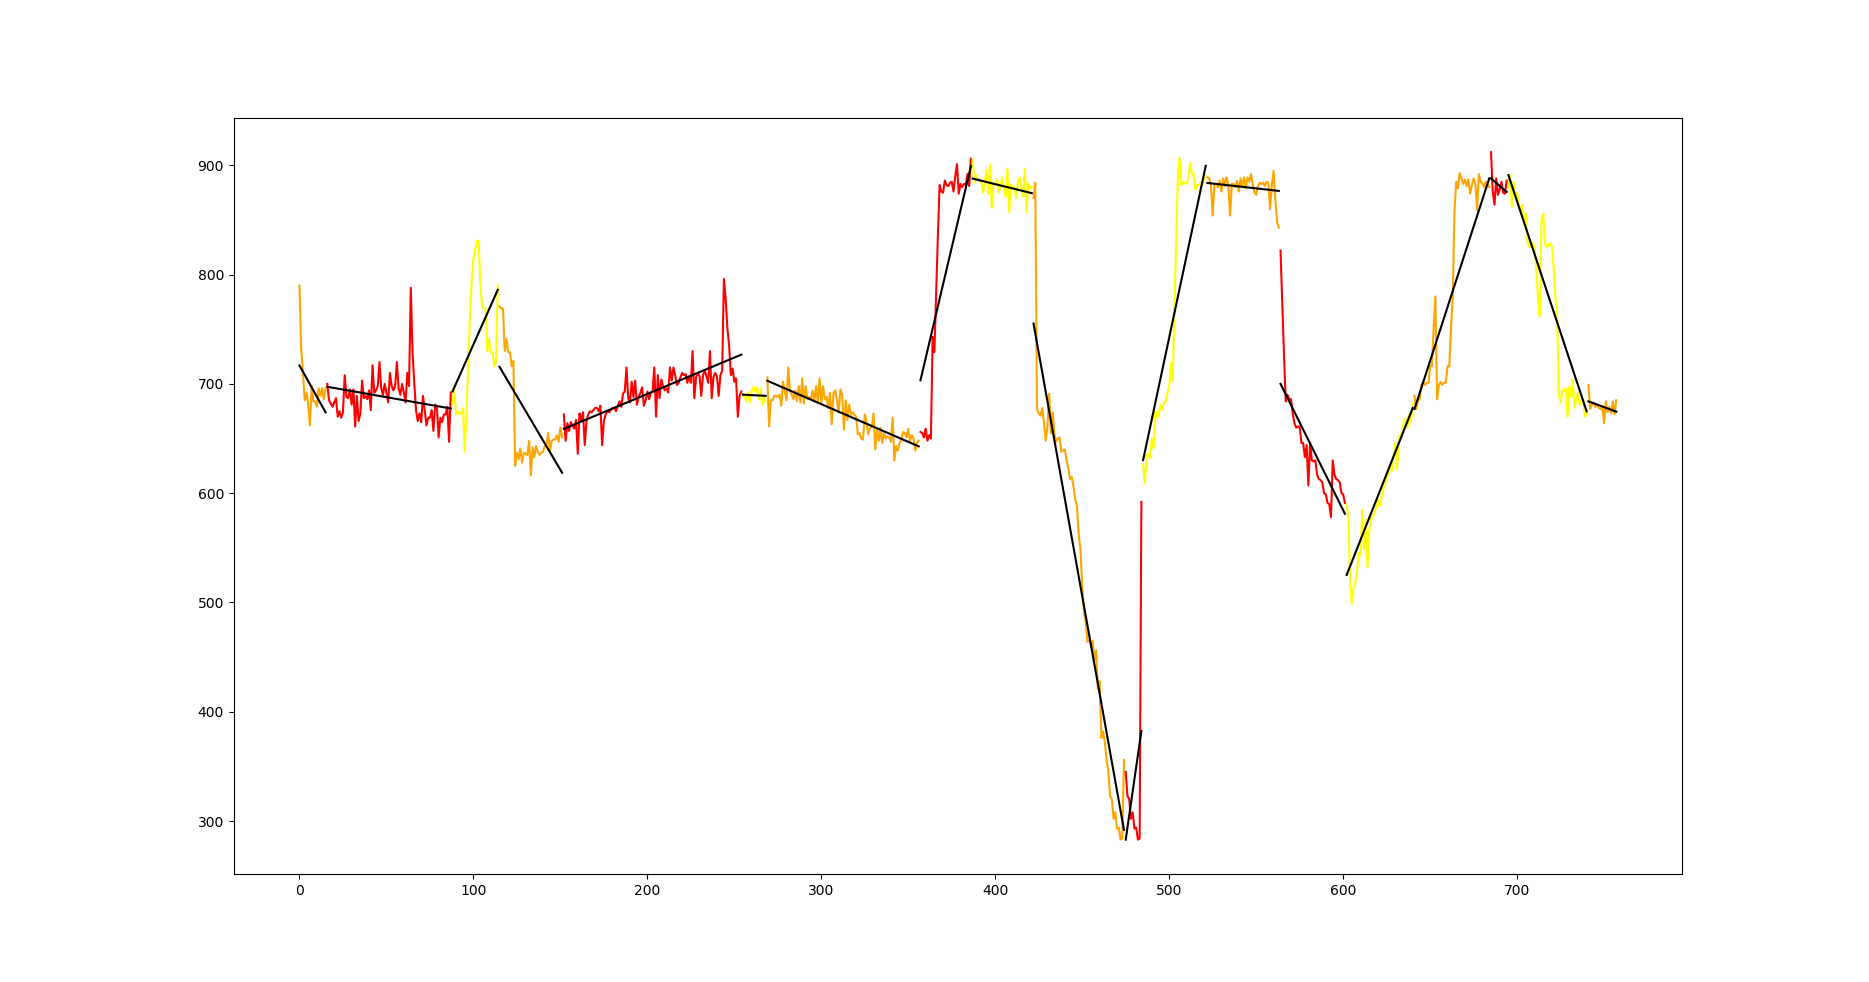
\includegraphics[width=0.8\textwidth]{img/artefacts.png}
    \end{center}
\end{frame}

% ---- CLASSIFIER ---- %
\begin{frame}\frametitle{Classification: classifier}
    \begin{itemize}
        \item Based on set of linear regression classifiers.
            \begin{center}
                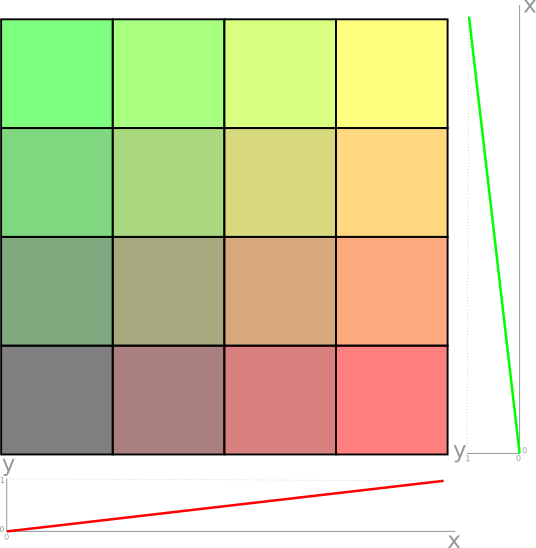
\includegraphics[width=0.3\textwidth]{img/area.png}
            \end{center}
            
        \item Spatial model of sensed area.
            \begin{center}
                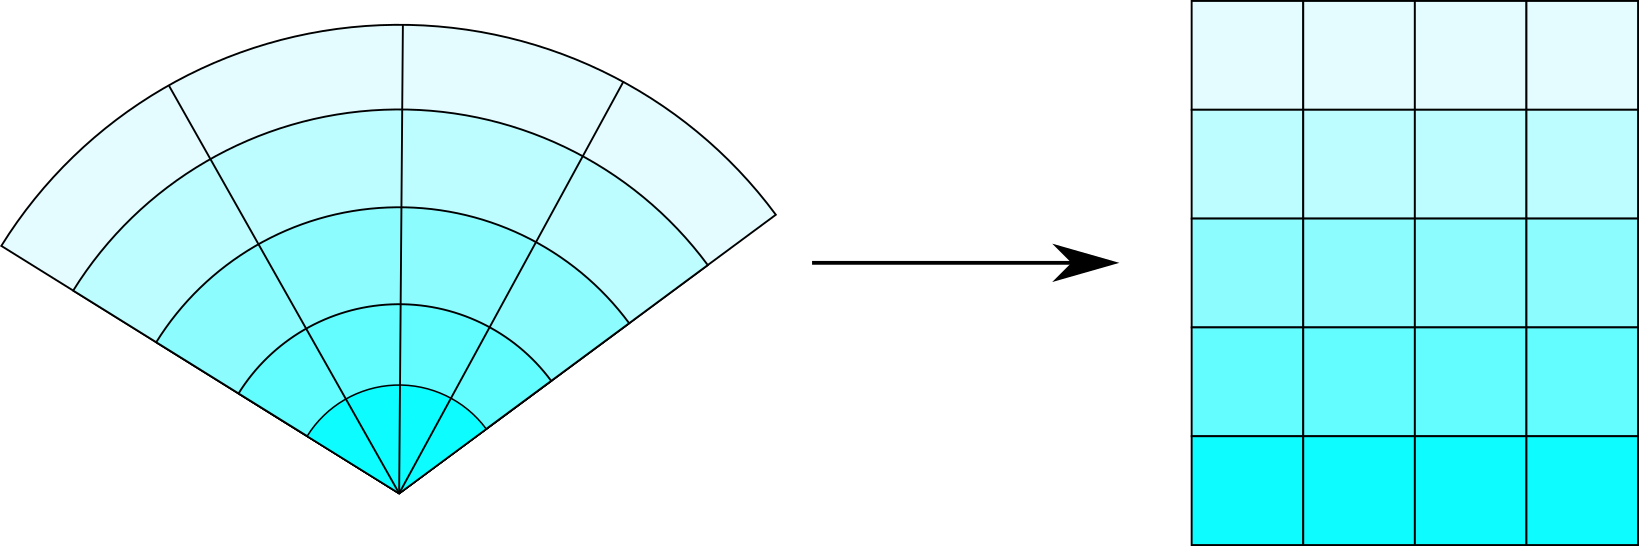
\includegraphics[width=0.65\textwidth]{img/circularsector.png}
            \end{center}

    \end{itemize}
\end{frame}

% ---- TRAINING ---- %
\begin{frame}\frametitle{Classification: training}
    \begin{center}
        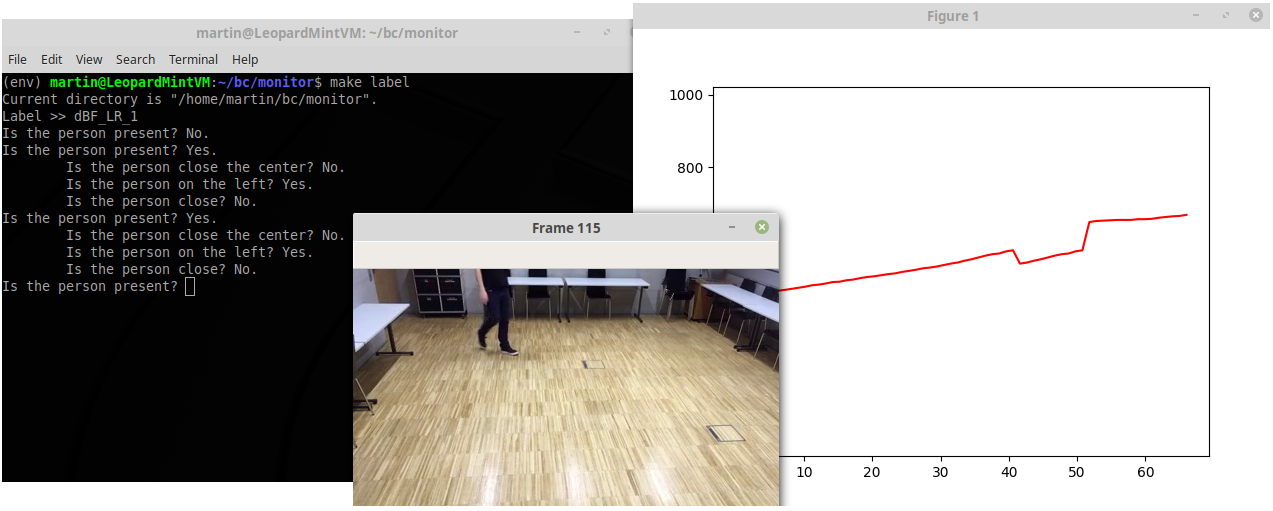
\includegraphics[width=1\textwidth]{img/labelling.png}
    \end{center}
\end{frame}

% ---- POSTPROCESSING ---- %
\begin{frame}\frametitle{Classification: postprocessing}
    \begin{itemize}
        \item For \emph{localization} cluster analysis is used.
            \begin{itemize}
                \item K-means
                \item Medoids (PAM)
            \end{itemize}
        \item \emph{Count of people} by minimal within-cluster sum of squares.
    \end{itemize}
\end{frame}

% ---- IMPLEMENTATION ---- %
% ---- SENSOR DEVICE ---- %
%\begin{frame}\frametitle{Implementation: sensor device}
%    \begin{itemize}
%        \item B+B Sensors: PIR STD
%            \begin{center}
%                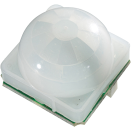
\includegraphics[width=0.15\textwidth]{img/pirstd.png}
%            \end{center}
%        \item NodeMCU (C++/Arduino)
%            \begin{itemize}
%                \item ESP8266 (WiFi)
%                \item mDNS, HTTP
%            \end{itemize}
%            \begin{center}
%                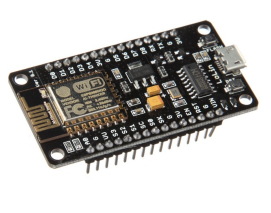
\includegraphics[width=0.25\textwidth]{img/nodemcu.png}
%            \end{center}
%        \item Communication with server via multicast
%    \end{itemize} 
%\end{frame} 

% ---- CLASSIFIER ---- %
%\begin{frame}\frametitle{Implementation: classification server}
%    \begin{itemize}
%        \item Python3
%            \begin{itemize}
%                \item NumPy, SciPy, scikit
%                \item MatPlotLib, PySerial
%            \end{itemize}
%        \item Linux, Bash
%    \end{itemize}
%\end{frame}

% ---- RESULTS ---- %
\begin{frame}\frametitle{Results}
    \begin{itemize}
        \item Posterior probability [\%] 
    \begin{center}
        \begin{tabular}{|c|c c c c|} \hline
            \textbf{Aspect} & \textbf{Presence} & \textbf{Distance} & \textbf{Center}       & \textbf{Left} \\ \hline
            Positive rate   & $75.972$          & $75.785$          & $63.725$              & $49.263$            \\
            Negative rate   & $86.542$          & $69.793$          & $53.436$              & $59.327$            \\ \hline
        \end{tabular}
    \end{center}
        \item Possible improvements
            \begin{itemize}
                \item Labelling
                \item Multiple sensors
            \end{itemize}
    \end{itemize}

\end{frame}


% ---- END ---- %
\bluepage{Thank You For Your Attention !}

\end{document}
